\section{\ours{} \raisebox{-.6ex}{
\includegraphics[width=0.6cm]{figures/logos/csmgym.png}}\,%
}

本节介绍 \ours{} 的设计和构建，包括领域选择、沙箱环境、\Cref{subsec:construction} 中的任务形式，以及 \Cref{subsec:statistics} 中的数据集统计。

\begin{figure}[t]
 \centering
 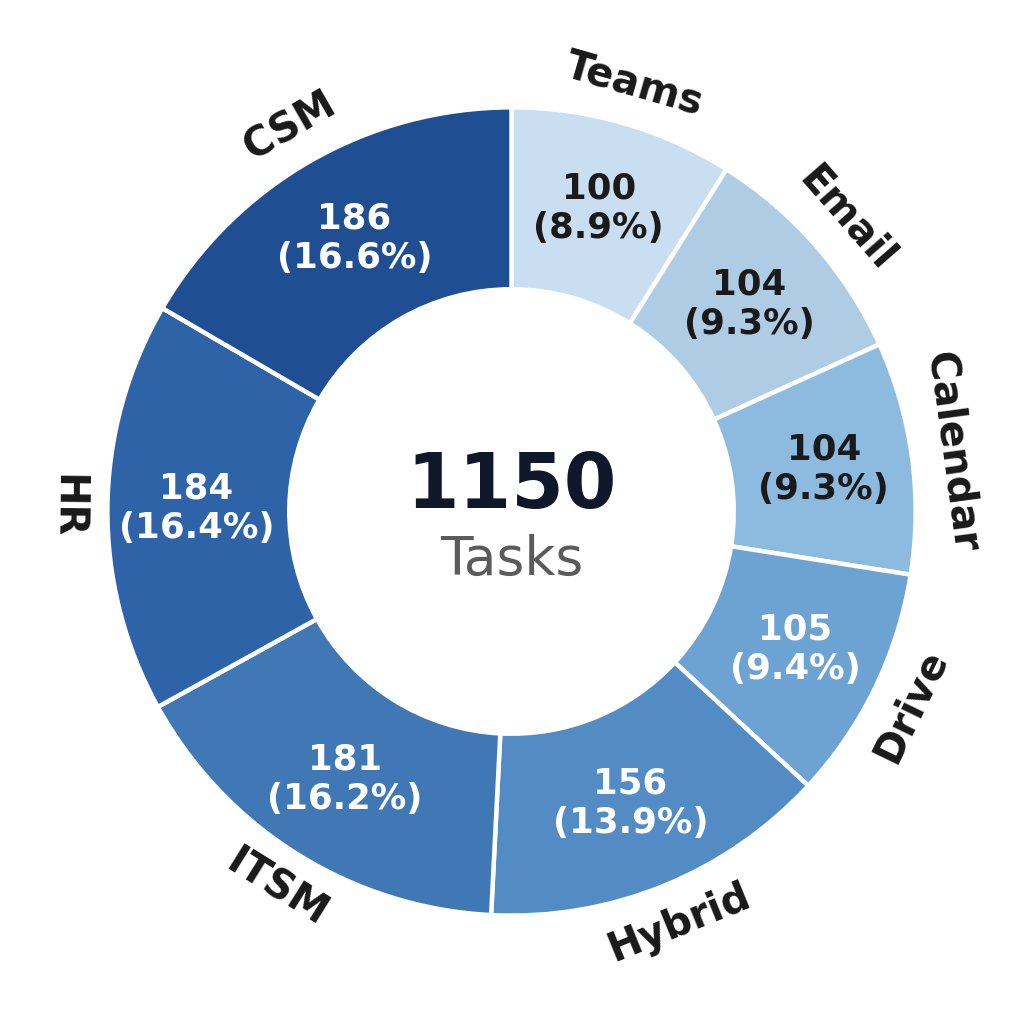
\includegraphics[width=0.7\linewidth]{figures/dataset/domain_distribution_donut.png}
 \caption{八个 \ours{} 领域的任务分布。}
 \label{fig:data_distribution}
\end{figure}

\subsection{\dataset 构建}
\label{subsec:construction}

\paragraph{领域选择}
我们与具有企业软件实操经验的领域专家（SME）协商后，依据三项原则选择领域：（i）与真实行业垂直领域相关；（ii）策略复杂度和数据敏感性具有多样性；（iii）有领域专家可编写并验证真实任务。据此得到两组互补的领域。

第一组由\textit{客户服务管理（CSM）}、\textit{人力资源（HR）}和\textit{信息技术服务管理（ITSM）}构成，是企业组织的运营骨干。这些领域几乎存在于每一种行业垂直领域，具有严格的流程合规、访问控制策略和高风险工作流，错误会带来切实后果。CSM 管理支持工单和服务协议的完整生命周期；HR 在严格隐私与流程规则下处理敏感员工数据；ITSM 覆盖包括事件管理和系统配置在内的后端 IT 运维。其重策略性质和现实复杂度使其适于压力测试约束感知规划。

第二组由\textit{Email}、\textit{Calendar}、\textit{Teams}和\textit{Drive}组成，涵盖所有企业每天使用的通用协作工具。智能体必须熟练掌握它们，才能充当有效的 AI 员工。尽管单独看来更简单，这些领域仍需要精密编排：\textit{Email} 处理复杂邮箱工作流，\textit{Calendar} 管理时间和资源访问策略，\textit{Teams} 管理协作工作空间，\textit{Drive} 则维护文件系统完整性与安全性。

最后，\textit{Hybrid} 要求在这些碎片化工具之间进行跨领域编排，智能体切换系统时必须保持上下文与数据完整性。八个领域共同覆盖完整的企业工作流谱系，从内部运营、面向客户的流程到协作基础设施，因而可同时评估专用和通用的智能体能力。

\paragraph{沙箱环境与数据生成}
我们与专业数据标注公司 Turing\footnote{https://www.turing.com} 合作，组建了由 160 多名贡献者构成的团队，其中包括构建环境的软件工程师，以及 CSM、ITSM、HR 等技术领域的主题专家。为提供可复现且真实的评测场地，我们开发了容器化 Docker 沙箱，其中承载领域特定的数据库、API 和工具执行层。该环境复现企业约束而不暴露专有基础设施。对每个领域，我们创建真实的数据库模式，并填充种子数据和用于访问、操作数据的工具。底层数据由 SME 从强现实视角设计；在官方产品文档和 SME 洞见的指引下，我们依据行业标准数据库模式建模真实的表结构、约束与工具。从固定的数据和工具种子出发，标注员会按每个任务的需要向环境扩展新表、模式和记录。

\paragraph{任务构建流水线}
任务创建遵循严格流水线，以确保高复杂度与对真实工作流的忠实性。在\textbf{场景设计}阶段，标注员依据明确的复杂度阈值构建具有挑战性的多步场景，考量工具调用数量、验证条件和状态依赖等维度（动作顺序对成功至关重要）、访问约束（例如 ``\textit{只有团队所有者可以创建私有频道}''）及其他策略冲突（用户请求与系统策略相冲突）。我们约束任务具有唯一最终状态，尽管到达它可能有多条有效路径。此外，我们设计了 30 个不可行任务：由于工具不足、显式策略违规或资源不可用，任务完成在设计上就是不可能的。对于每个任务，标注员也会更新沙箱，增加必要的表和工具。随后进入\textbf{真值执行与计划编写}阶段：标注员为每个任务提供细粒度的逐步计划，并在沙箱中手动执行以捕获黄金标准轨迹，记录每次调用的参数、响应和执行理由。标注员还会编写自然语言推理计划，将每个动作明确地锚定在系统约束、用户请求和可用工具上。计划会引用系统提示词中的策略，并解释顺序依赖，从而使任务在给定上下文中得到完整依据。

我们实施\textbf{以结果为中心的验证}：标注员编写可执行 SQL 验证脚本，在任务完成后检查环境最终状态。这样我们评估的是\emph{结果}而不是僵化的动作序列，因而允许多条有效的解题路径。评测会检查必需条件（\emph{是否达成目标？}）、完整性约束（\emph{是否遵守外键约束？}）、权限合规（\emph{智能体是否避免未授权动作？}）及其他副作用。最后，我们进行多轮\textbf{质量保证}：复审标注员（包括作者）评估给定初始状态和可用工具时任务是否可行，指令是否清晰完整且不依赖外部依赖或领域知识，验证脚本的正确性和覆盖率，以及真值计划、指令和验证脚本的流畅性与连贯性。

\subsection{数据集统计}
\label{subsec:statistics}

\paragraph{任务统计}
\dataset 在 1,150 个任务上评估智能体，这些任务旨在复现真实企业操作的深度，其中包括 30 个不可行任务，用来测试智能体能否正确拒绝无法满足的请求。动作空间广泛而多样，跨领域含 512 个唯一工具；各领域工具集从 Calendar 的 37 个到 ITSM 的 93 个不等。专家人工轨迹平均为 9.15 步，规划跨度在领域间显著不同：Email 平均 6.2 步，CSM 平均 12.1 步，HR 最长可达 34 步。除长度外，任务的约束也很密集：平均每个任务要求满足 5.3 个不同的验证条件，最复杂的场景需要解决 44 个条件。

\paragraph{环境统计}
我们的沙箱环境建模了一个高度互连的数据生态，八个领域共含 164 张唯一数据库表。平均每个任务与由 24.9 张表构成的子图交互，Hybrid 场景中最多达到 73 张。这意味着智能体必须在一个大型、部分可观测的数据图上推理，才能正确执行任务。每个任务平均涉及 3,443 行数据库记录；在 CSM 等数据密集领域中超过 10,000 行。为量化关系复杂度，我们测量每张表的平均外键（FK）数量。依赖程度很高，Calendar 平均为 1.1 个外键，HR 为 2.4 个，整体均值约为 1.7，超过先前基准的关系密度（见表~\ref{tab:related_works_comparison}）。更高的外键密度意味着智能体在构造有效工具参数时必须解析更多表间依赖，因此参照完整性成为关键挑战。
